\part{Klasifikace příznaků}

Nalézt korespondující dvojice měřených a referenčních svazků pouze pomocí směru svazků je prakticky nemožné. Víme, že u měřených svazků můžeme kromě směru určit zářivý tok a detekovat ocásky (kapitola \ref{sec:beam parameters}).   

Prozkoumáme parametry referenčních a měřených svazků s cílem definovat závislost parametrů pomocí jednoduché funkce. Nalezení závislosti parametrů zjednoduší úlohu korespondence svazků.  


\section{Ground truth}

Abychom mohli hledat závislosti mezi parametry měřených a referenčních svazků, potřebujeme získat data  s korespondujícími svazky. Toho dosáhneme tak, že ručně upravujeme množinu korespondencí a optimalizujeme náklon faset. Proces ručního přiřazování svazků ukončíme, když nalezneme optimální náklon faset, který zajišťuje maximální shodu měřených a referenčních svazků. Tyto korespondence považujeme za správné.    

Ručně určené korespondence označujeme výrazem "\textit{ground truth}" podobně jako v oblasti strojového učení, kde slouží jako přesná data v trénovací množině pro určení statistických modelů. Použití výrazu "\textit{ground truth}" je ovšem v našem případě sporné, neboť určení množiny korespondencí závisí na osobě, která tato úlohu provádí. To, co v našem případě označujeme jako "\textit{ground truth}", je množina, o které se domníváme, že by měla obsahovat správné korespondence svazků, ale v našem případě nemůžeme s naprostou jistotou tvrdit, že tomu tak je. 

\section{Změna zářivého toku se změnou parametrů kamene}
\label{sec: zmena_tok }

	Chceme zjistit, jak je zářivý tok svazků závislý na změně parametrů faset. 

	Máme k dispozici 27 snímků, které zachycují 9 různých kamenů typu \textit{viva12}. Při určení "\textit{ground truth}" jsme zároveň nalezli optimální matematické modely kamenů. Vezmeme si postupně každý s těchto modelů a měníme náklon normály vybrané fasety o jeden stupeň ve čtyřech kolmých směrech. Nakonec normálu vrátíme zpět na původní hodnotu. Takto nakloníme normály všech 14-ti faset kamene.
	
	Nakloněním normály fasety vznikne nový model kamene. Pro tento model pomocí LADOKu  vyřešíme parametry svazků. Pokud se zářivý tok svazku od původního modelu změnil, zapamatujeme si jeho hodnotu. Pro jednotlivý svazek dostaneme vektor hodnot zářivého toku $\vv{\phi_e}$. 
	
	 Abychom mohli porovnat změnu zářivého toku, který se může u svazků řádově lišit, vyjádříme změnu toku pomocí variačního koeficientu $c_v$. Variační koeficient je výsledkem podílu směrodatné odchylky a střední hodnoty vektoru $\vv{\phi_e}$. 
	 
	 \begin{equation}	 
	 c_v = \frac{\sigma(\vv{\phi}_e)}{E(\vv{\phi}_e)}\,. 
	 \end{equation}
	 
Určíme variační koeficient všech referenčních svazků se známými korespondujícími svazky a výsledek zaneseme do histogramu \ref{fig: flux_var_coeff}. V histogramu vidíme, že existuje nezanedbatelný počet svazků, pro které změna náklonu fasety o \SI{1}{\degree} znamená změnu zářivého toku o více než polovinu původní hodnoty. Je zřejmé, že obdobně se bude měnit zářivý tok svazků při posunu fasety. 

 Výsledek naznačuje, že nebude snadné nalézt funkci, která by definovala vztah mezi zářivým tokem referenčních a měřených svazků.  

\begin{figure}[htps]
\centering
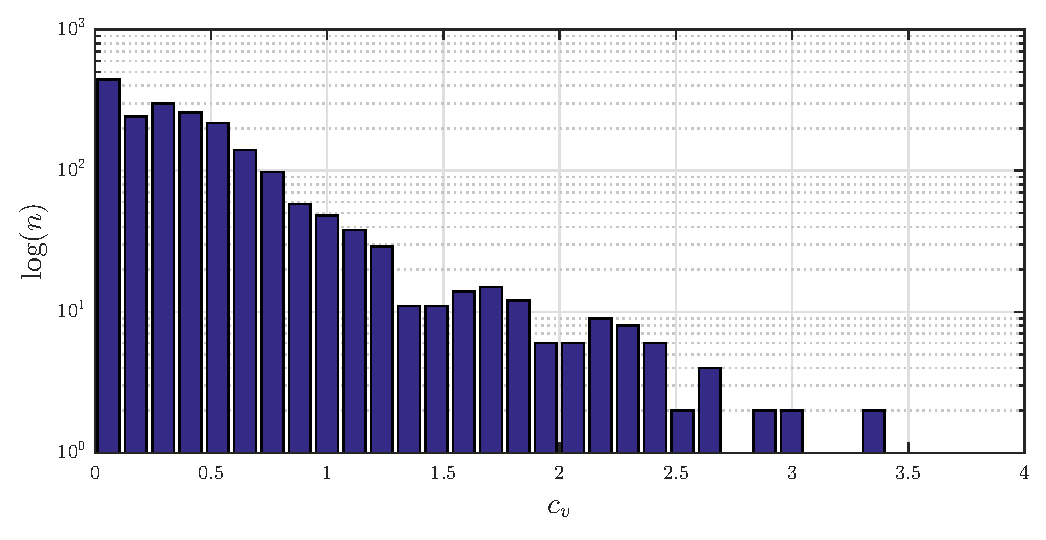
\includegraphics[width = \textwidth]{flux_var_coeff.eps}
\caption{Histogram variačního koeficientu zářivého toku svazků pro data z 27 snímků kamene \textit{viva12}.}
\label{fig: flux_var_coeff}
\end{figure}



\section{Závislost zářivého toku}
	Broušený kámen je ozářen laserovým svazkem o vlnové délce \SI{670}{\nano\metre}. Při průchodu světelného svazku kamenem se část záření absorbuje a přemění se na teplo. Absorpce záření závisí na odstínu kamene, proto si vybereme kameny stejného odstínu. V našem případě zvolíme odstín \textit{Hyacint}, který se vyznačuje nízkou absorpcí zdrojového svazku. 
	
	Korespondující svazky jsme určili pro 4 kameny odstínu \textit{Hyacint}, kde každý svazek byl 3$\times$ s různou rotací umístěn do měřicí soustavy. S korespondencemi z 12 snímků pracujeme jako s celkem a dostaneme množinu uspořádaných dvojic měřených a referenčních svazů. 
	
	Měřené svazky charakterizuje zářivý tok $\vv{\phi}_{e_m}$ a referenční svazky zářivý tok $\vv{\phi}_{e_r}$. Cílem je nalézt funkci $h$, pro kterou
	
	\begin{equation}	
		\phi_{e_r} = h \left( \phi_{e_m} \right) \,.
		\label{eq: fi_fi}
	\end{equation}

Abychom mohli porovnat data z více měření, vyjádříme si zářivý tok měřených svazků jako jejich poměr ku součtu zářivého toku všech měřených svazků v jednotlivém snímku. 

Závislost $\phi_{e_r} =  f\left( \phi_{e_m} \right)$ vyneseme do grafu \ref{fig: flux_depend2}, kde jsou vykresleny pouze svazky s variačním koeficientem $c_v$ menším než $0.5$. Do grafu zároveň zakreslíme hranice $\mathbf{b_0}$ a $\mathbf{b_1}$ vymezující oblast, kde se nachází většina svazků.

  Výsledek není příliš optimistický. Data v grafu jsou příliš rozptýlena na to, abychom mohli nalézt spolehlivou funkci popisující závislost \ref{eq: fi_fi}. Důvodů může být hned několik. 

Víme, že v modelu kamene nejsou postihnuty všechny skutečnosti ovlivňující velikost zářivého toku stop. Můžeme zmínit například to, že v modelu není zahrnuta čistota materiálu, která nemusí a prakticky ani není v celém materiálu konstantní. Nedokonalé proleštění fasety ovlivňuje rozptylové parametry světelného svazku. Změna parametrů fasety vede ke změně plochy fasety, tedy i ke změně plochy svazku, který je omezen hranou této fasety. Malá změna parametrů fasety může vést k velké změně zářivého toku svazku, což jsme si ukázali v kapitole \ref{sec: zmena_tok }. Tyto a další vlastnosti v konečném důsledku vyústí v chybu údaje na y-ové ose grafu \ref{fig: flux_depend2}.

Na druhé straně musíme počítat s nejistotou určení zářivého toku detekovaných svazků vznikající při extrakci parametrů svazků z obrazu. Mezi zásadní problémy patří šum, překrývání stop, difuzní odrazivost svazků či odhad pozadí snímku.  

\begin{figure}[htps]
\centering
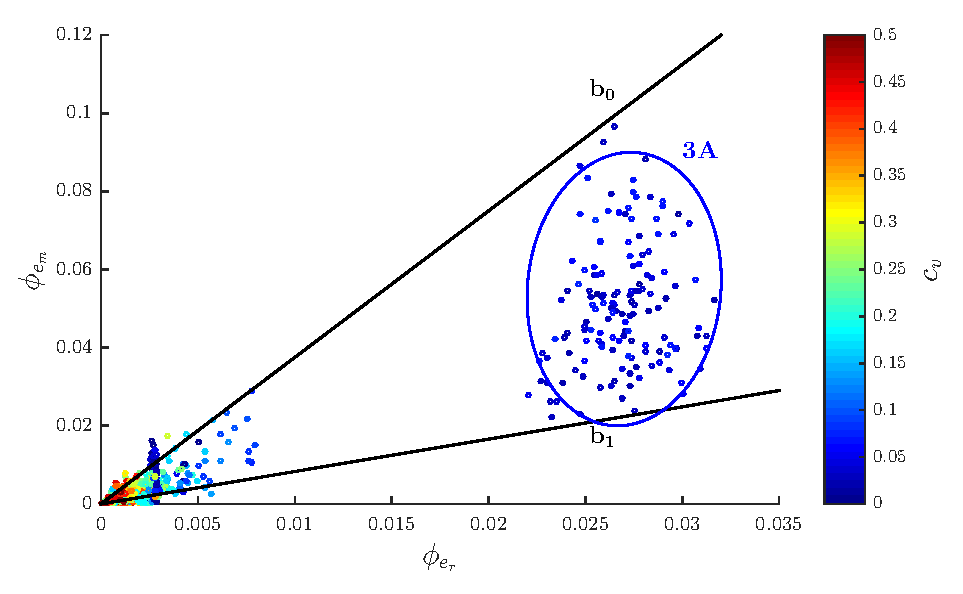
\includegraphics[width = 0.8\textwidth]{flux_depend2.eps}
\caption{Závislost zářivého toku referenčních svazků na velikosti zářivého toku měřených svazků. Zobrazeny jsou pouze svazky s variačním koeficientem zářivého toku větším než $0.5$. Zakresleny jsou vymezovací hranice $\mathbf{b_0}$ a $\mathbf{b_1}$. Výsledky pro odstín \textit{Hyacint}.}
\label{fig: flux_depend2}
\end{figure}

\begin{figure}[htps]
\centering
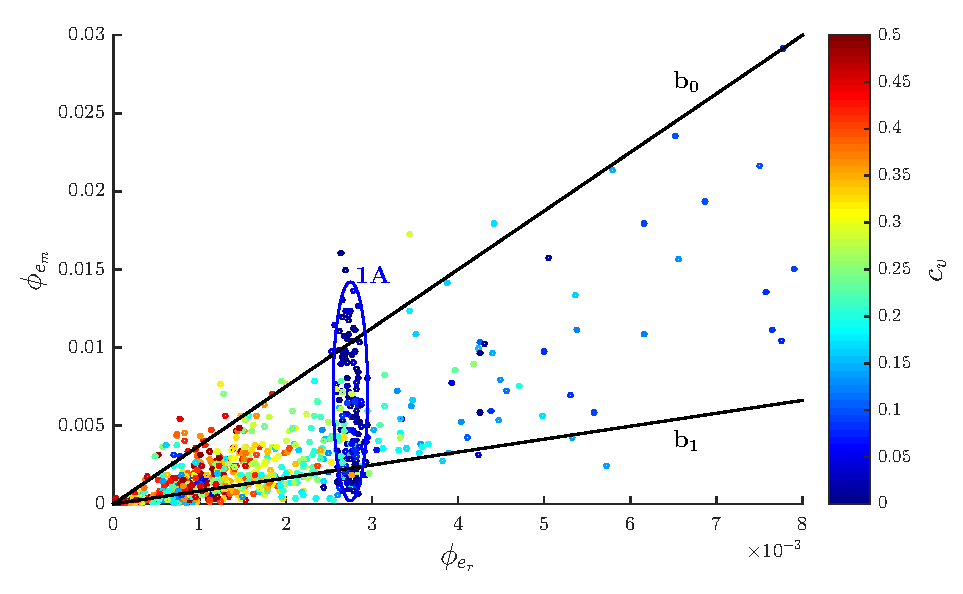
\includegraphics[width = 0.8\textwidth]{flux_depend1.eps}
\caption{Detail obrázku \ref{fig: flux_depend2}. Vynechány jsou svazky třídy \textbf{3A}.}
\label{fig: flux_depend1}
\end{figure}


Ve grafu \ref{fig: flux_depend2} jsou patrné shluky bodů, které přesto, že mají referenční zářivý tok podobné velikosti se velikost detekovaného zářivého toku znatelně liší. Při detailnějším pohledu zjistíme, že se jedná o stopy třídy (\textbf{1A} a \textbf{3A}). Tyto svazky se navíc vyznačují téměř nulovým variačním koeficientem zářivého toku. Pro třídu \textbf{1A} můžeme velké odchylky vysvětlit tím, že povrch kamene byl až matný a  odrážel tak více světla, než jsme očekávali. 

\section{Závislost parametrů ocásků}

	Zajímáme se to, jak může přispět znalost ocásků měřených s referenčních svazků k nalezení korespondující dvojice.  

  Korespondující ocásky nalezeme pomocí jednoduchého algoritmu založeného na podobnosti směru ocásků korespondujících stop a výsledek ručně upravíme. Máme k dispozici data korespondujících ocásků pro 25 snímků celkem deseti kamenů \textit{viva12}. 
	
	Ocásky parametrizujeme pomocí velikosti $\rho$ a směrového úhlu $\phi$. Z korespondujících ocásků získáme parametry měřených ocásků $\vv{\rho}_m$ a $\vv{\varphi}_m$ a k nim odpovídající parametry $\vv{\rho}_r$ a $\vv{\varphi}_r$.
	

\subsection{Směrový úhel}
 U směrového úhlu potřebujeme vědět, do jaké míry souhlasí směr měřeného a směr referenčního svazku. Vypočítáme rozdíl směrových úhlů $\Delta\vv{\phi}$ a vyneseme do grafu \ref{fig: tail_depend1} rozložení pravděpodobnosti.  
 
 \begin{equation}
 \Delta\vv{\phi} = \vv{\varphi}_m - \vv{\varphi}_r\,.
 \end{equation}
  
\begin{figure}[htps]
\centering
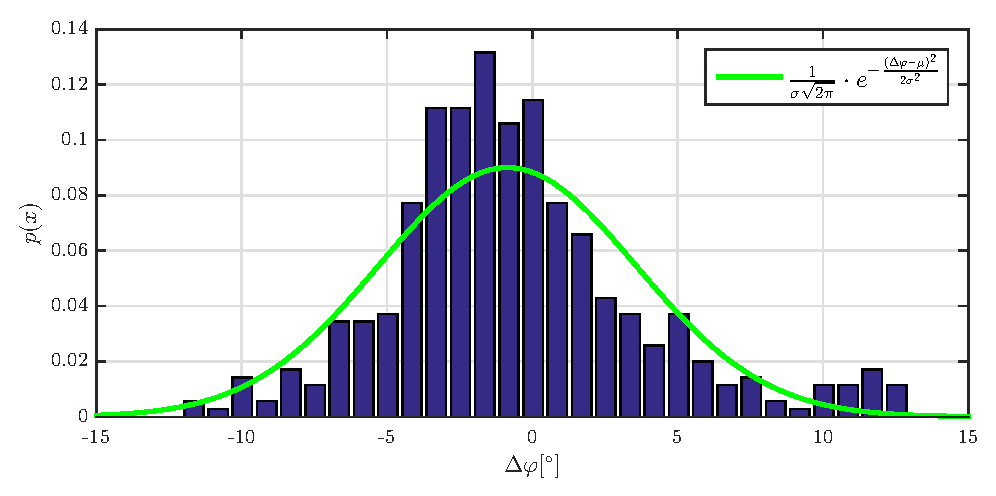
\includegraphics[width = 0.8\textwidth]{tails_gauss.eps}
\caption{Odhad pravděpodobnostní funkce rozdílu směrového úhlu mezi měřenými a referenčními ocásky. Aproximace Gaussovou křivkou s parametry $\sigma = $ \SI{4.43}{\degree} a $\mu = $ \SI{-0.86}{\degree}. }
\label{fig: tail_depend1}
\end{figure}

Pravděpodobnostní rozdělení na obr. \ref{fig: tail_depend1} lze aproximovat Gaussovu funkcí

\begin{equation}
f(\Delta\varphi) = \frac{1}{\sigma\sqrt{2\pi}}\cdot e^{-\frac{\left(\Delta\varphi - \mu\right)^2}{2\sigma^2}}\, 
\end{equation}
s rozptylem $\sigma =  $ \SI{4.43}{\degree} = \SI{0.077}{\radian} a střední hodnotou $\mu = $ \SI{-0.86}{\degree} = \SI{-0.15}{\radian}. Tato funkce může sloužit jako základ pro určení podobnostní ocásků.   

\subsection{Velikost}
	Vykreslili jsme si závislost velikosti referenčních ocásků na velikosti měřených ocásků. V grafu \ref{fig: tail_depend2} jsou pouze náhodně vybrané vzorky závislosti $\rho_r = f(\rho_m)$  , kde $\rho_m = \dfrac{\rho_m}{max{\vv{\rho}_m}}$. Naměřené velikosti ocásků se zdají být v souvislostí s velikostí referenčních ocásků takřka nahodilé. Nejsme schopni nalézt funkci $f$, která by popisovala závislost $\rho_r = f(\rho_m)$.
	
	\begin{figure}[htps]
\centering
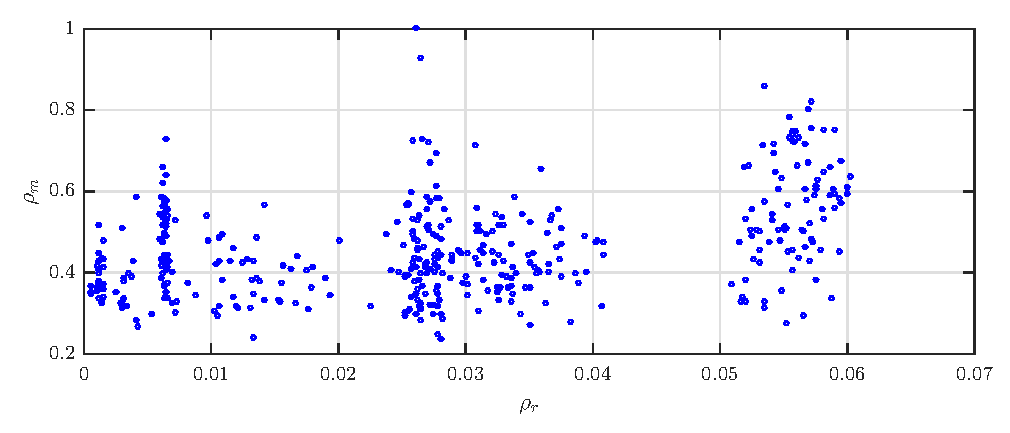
\includegraphics[width = 0.8\textwidth]{tails_rho.eps}
\caption{Závislost velikosti referenčních ocásků $\rho_r$ na velikosti měřených ocásků $\rho_m$ pro náhodně vybranou podmnožinu korespondujících ocásků.}
\label{fig: tail_depend2}
\end{figure}

\clearpage